\documentclass[12pt,a4paper]{article}

% --- Paquetes esenciales ---
\usepackage[utf8]{inputenc}
\usepackage[T1]{fontenc}
\usepackage[spanish,es-tabla]{babel}
\usepackage{geometry}
\geometry{top=2.5cm, bottom=2.5cm, left=3cm, right=2.5cm}

\usepackage{amsmath,amssymb}
\usepackage{graphicx}
\usepackage{booktabs}
\usepackage{array}
\usepackage{tabularx}
\usepackage{caption}
\usepackage{hyperref}
\hypersetup{
  colorlinks=true,
  linkcolor=blue,
  citecolor=blue,
  urlcolor=blue
}
\usepackage{parskip}
\usepackage{setspace}
\onehalfspacing

% --- Datos del artículo ---
\title{Simulación de Eventos Discretos del\\Proceso de Desarrollo Software\\en Cascada (Waterfall)}
\author{Departamento de Ingeniería — Universidad XXX}
\date{\today}

\begin{document}

\maketitle
\thispagestyle{empty}

% ============================================================
\section{Metodología}
\label{sec:metodologia}
% ============================================================

El modelo conceptual del proceso waterfall se implementó en FlexSim como una simulación de eventos discretos, utilizando datos históricos reales correspondientes a 365 días de operación de un equipo de desarrollo software. El modelo captura el flujo secuencial de trabajo, los mecanismos de retroalimentación por retrabajo, las interrupciones por hotfix urgentes y la dinámica de recursos limitados.

\subsection{Arquitectura del Proceso}

El flujo de trabajo sigue cinco fases secuenciales sin solapamiento, reflejando el modelo waterfall clásico: \textit{Requisitos} $\rightarrow$ \textit{Diseño} $\rightarrow$ \textit{Implementación} $\rightarrow$ \textit{Verificación (QA)} $\rightarrow$ \textit{Mantenimiento}. A diferencia de metodologías ágiles, no existe solapamiento entre fases ni iteraciones planificadas: cada tarea avanza linealmente a través de las etapas, salvo cuando se activan los mecanismos de retrabajo descritos en la Sección~\ref{subsec:feedback}.

Cada fase del modelo incorpora parámetros estocásticos obtenidos del análisis de datos históricos (Sección~\ref{subsec:resultados-entrada}). La Figura~\ref{fig:diagrama-proceso} presenta el diagrama completo del modelo conceptual, incluyendo distribuciones de probabilidad, recursos y puntos de decisión.

\begin{figure}[htbp]
  \centering
  \includegraphics[width=\textwidth]{diagrama-waterfall.png}
  \caption{Diagrama del modelo conceptual del proceso waterfall en FlexSim. Se indican las cinco fases secuenciales, las flechas de retrabajo (rojo punteado), el mecanismo de interrupción por hotfix, los pools de recursos y las distribuciones estocásticas asociadas a cada fase.}
  \label{fig:diagrama-proceso}
\end{figure}

\subsection{Mecanismos de Retroalimentación}
\label{subsec:feedback}

El modelo incorpora tres mecanismos de retroalimentación que desvían tareas de su flujo lineal:

\begin{enumerate}
  \item \textbf{Fallo en QA}: cuando una tarea no supera la verificación, retorna a la fase de Implementación para su corrección. Este evento ocurre con probabilidad $p = 0{,}2411$, estimada a partir de los 88 días con retrabajo registrados en el histórico.
  \item \textbf{Cambio de requisitos}: durante la fase de Mantenimiento pueden surgir nuevas solicitudes que requieren retornar a la fase de Requisitos. La probabilidad observada es $p = 0{,}1425$ (52 días en 365).
  \item \textbf{Bug en mantenimiento}: la detección de errores en producción genera retrabajo directo sobre Implementación. La tasa de bugs sigue una distribución Poisson con $\lambda = 2{,}89$ bugs/día.
\end{enumerate}

\subsection{Interrupción por Hotfix Urgente}

El modelo implementa un mecanismo de interrupción con prioridad máxima para hotfix urgentes. Cuando se activa este evento (Bernoulli, $p = 0{,}074$), una tarea de hotfix se inserta al inicio de la cola de Implementación, desplazando el trabajo en curso. Este mecanismo representa el 10{,}68\% del total de tareas procesadas.

\subsection{Restricción de Recursos}

Los recursos del modelo simulan la capacidad real del equipo:
\begin{itemize}
  \item \textbf{Developers}: entre 3 y 7 recursos simultáneos ($\mu = 5{,}1$), con ausencia aleatoria Bernoulli($p = 0{,}104$).
  \item \textbf{QA}: entre 1 y 3 recursos ($\mu = 2{,}1$), con saturación por cola de espera Bernoulli($p = 0{,}181$).
\end{itemize}

La saturación de QA constituye el principal cuello de botella del sistema: cuando la cola supera la capacidad de procesamiento, las tareas completadas desde Implementación se acumulan, generando bloqueos que se propagan aguas arriba.

\subsection{Elementos Estocásticos}

Las variables aleatorias del modelo se ajustaron a partir de datos históricos mediante pruebas de bondad de ajuste Kolmogorov--Smirnov. La Tabla~\ref{tab:distribuciones} presenta las distribuciones seleccionadas y sus parámetros.

\begin{table}[htbp]
  \centering
  \caption{Distribuciones de probabilidad ajustadas para las variables del modelo de simulación.}
  \label{tab:distribuciones}
  \begin{tabular}{lll}
    \toprule
    \textbf{Variable} & \textbf{Distribución} & \textbf{Parámetros} \\
    \midrule
    Llegadas (tareas/día) & Normal & $\mu = 11{,}57$, $\sigma = 3{,}38$ \\
    Desarrollo (horas) & Weibull & $k = 2{,}17$, $\lambda = 6{,}21$, loc $= 5{,}63$ \\
    QA (horas) & Normal & $\mu = 4{,}01$, $\sigma = 1{,}15$ \\
    Retrabajo (horas) & Weibull & $k = 3{,}78$, $\lambda = 6{,}21$, loc $= -0{,}40$ \\
    Retrabajo (tasa) & Bernoulli & $p = 0{,}2411$ \\
    Bugs (cant/día) & Poisson & $\lambda = 2{,}89$ \\
    Saturación QA & Bernoulli & $p = 0{,}181$ \\
    Ausencia recurso & Bernoulli & $p = 0{,}104$ \\
    \bottomrule
  \end{tabular}
\end{table}

\subsection{Tipos de Tarea}

Las tareas se clasificaron en cuatro categorías según su naturaleza, con la siguiente distribución observada: \textit{Feature} (50{,}68\,\%), \textit{Bug} (20{,}55\,\%), \textit{Refactor} (18{,}08\,\%) y \textit{Hotfix} (10{,}68\,\%). Esta clasificación es relevante porque cada tipo de tarea presenta distintas probabilidades de activar retrabajo y distintos tiempos de procesamiento.

% ============================================================
\section{Resultados}
% ============================================================

\subsection{Resultados de Entrada: Análisis Estadístico e Histogramas}
\label{subsec:resultados-entrada}

El análisis de los datos históricos permitió caracterizar el comportamiento del proceso mediante frecuencias de eventos (Tabla~\ref{tab:frecuencias}) y probabilidades empíricas (Tabla~\ref{tab:probabilidades}). En total se registraron 4{.}223 tareas nuevas ($\mu = 11{,}57$/día), de las cuales 3{.}173 fueron completadas en el período. Se detectaron 81 bugs en QA y 88 días con retrabajo, lo que representa el 24{,}11\,\% del tiempo operativo.

\begin{table}[htbp]
  \centering
  \caption{Frecuencias de eventos observados durante los 365 días del histórico.}
  \label{tab:frecuencias}
  \begin{tabular}{lr}
    \toprule
    \textbf{Evento} & \textbf{Frecuencia} \\
    \midrule
    Tareas nuevas totales & 4{.}223 \\
    Tareas completadas & 3{.}173 \\
    Bugs detectados en QA & 81 \\
    Días con retrabajo & 88 \\
    Días con cambio de requisitos & 52 \\
    Días con hotfix urgente & 27 \\
    Días con saturación QA & 66 \\
    \bottomrule
  \end{tabular}
\end{table}

\begin{table}[htbp]
  \centering
  \caption{Probabilidades empíricas de eventos discretos en el proceso.}
  \label{tab:probabilidades}
  \begin{tabular}{lc}
    \toprule
    \textbf{Evento} & \textbf{Probabilidad} \\
    \midrule
    Retrabajo & 0{,}2411 \\
    Cambio de requisitos & 0{,}1425 \\
    Hotfix urgente & 0{,}0740 \\
    Saturación QA & 0{,}1808 \\
    Ausencia de recurso & 0{,}1041 \\
    Repriorización & 0{,}1781 \\
    \bottomrule
  \end{tabular}
\end{table}

La Figura~\ref{fig:analisis-visual} presenta un panel con seis visualizaciones que resumen los patrones detectados: estacionalidad mensual con variación significativa entre meses, ráfagas de actividad que superan en más de $2\sigma$ la media diaria, clústeres de retrabajo en días consecutivos (lo que sugiere dependencia temporal), y correlaciones relevantes entre volumen de tareas y completadas, entre complejidad y tiempo de desarrollo, y entre bugs y retrabajo. Adicionalmente se observó una tendencia semanal decreciente en la productividad.

\begin{figure}[htbp]
  \centering
  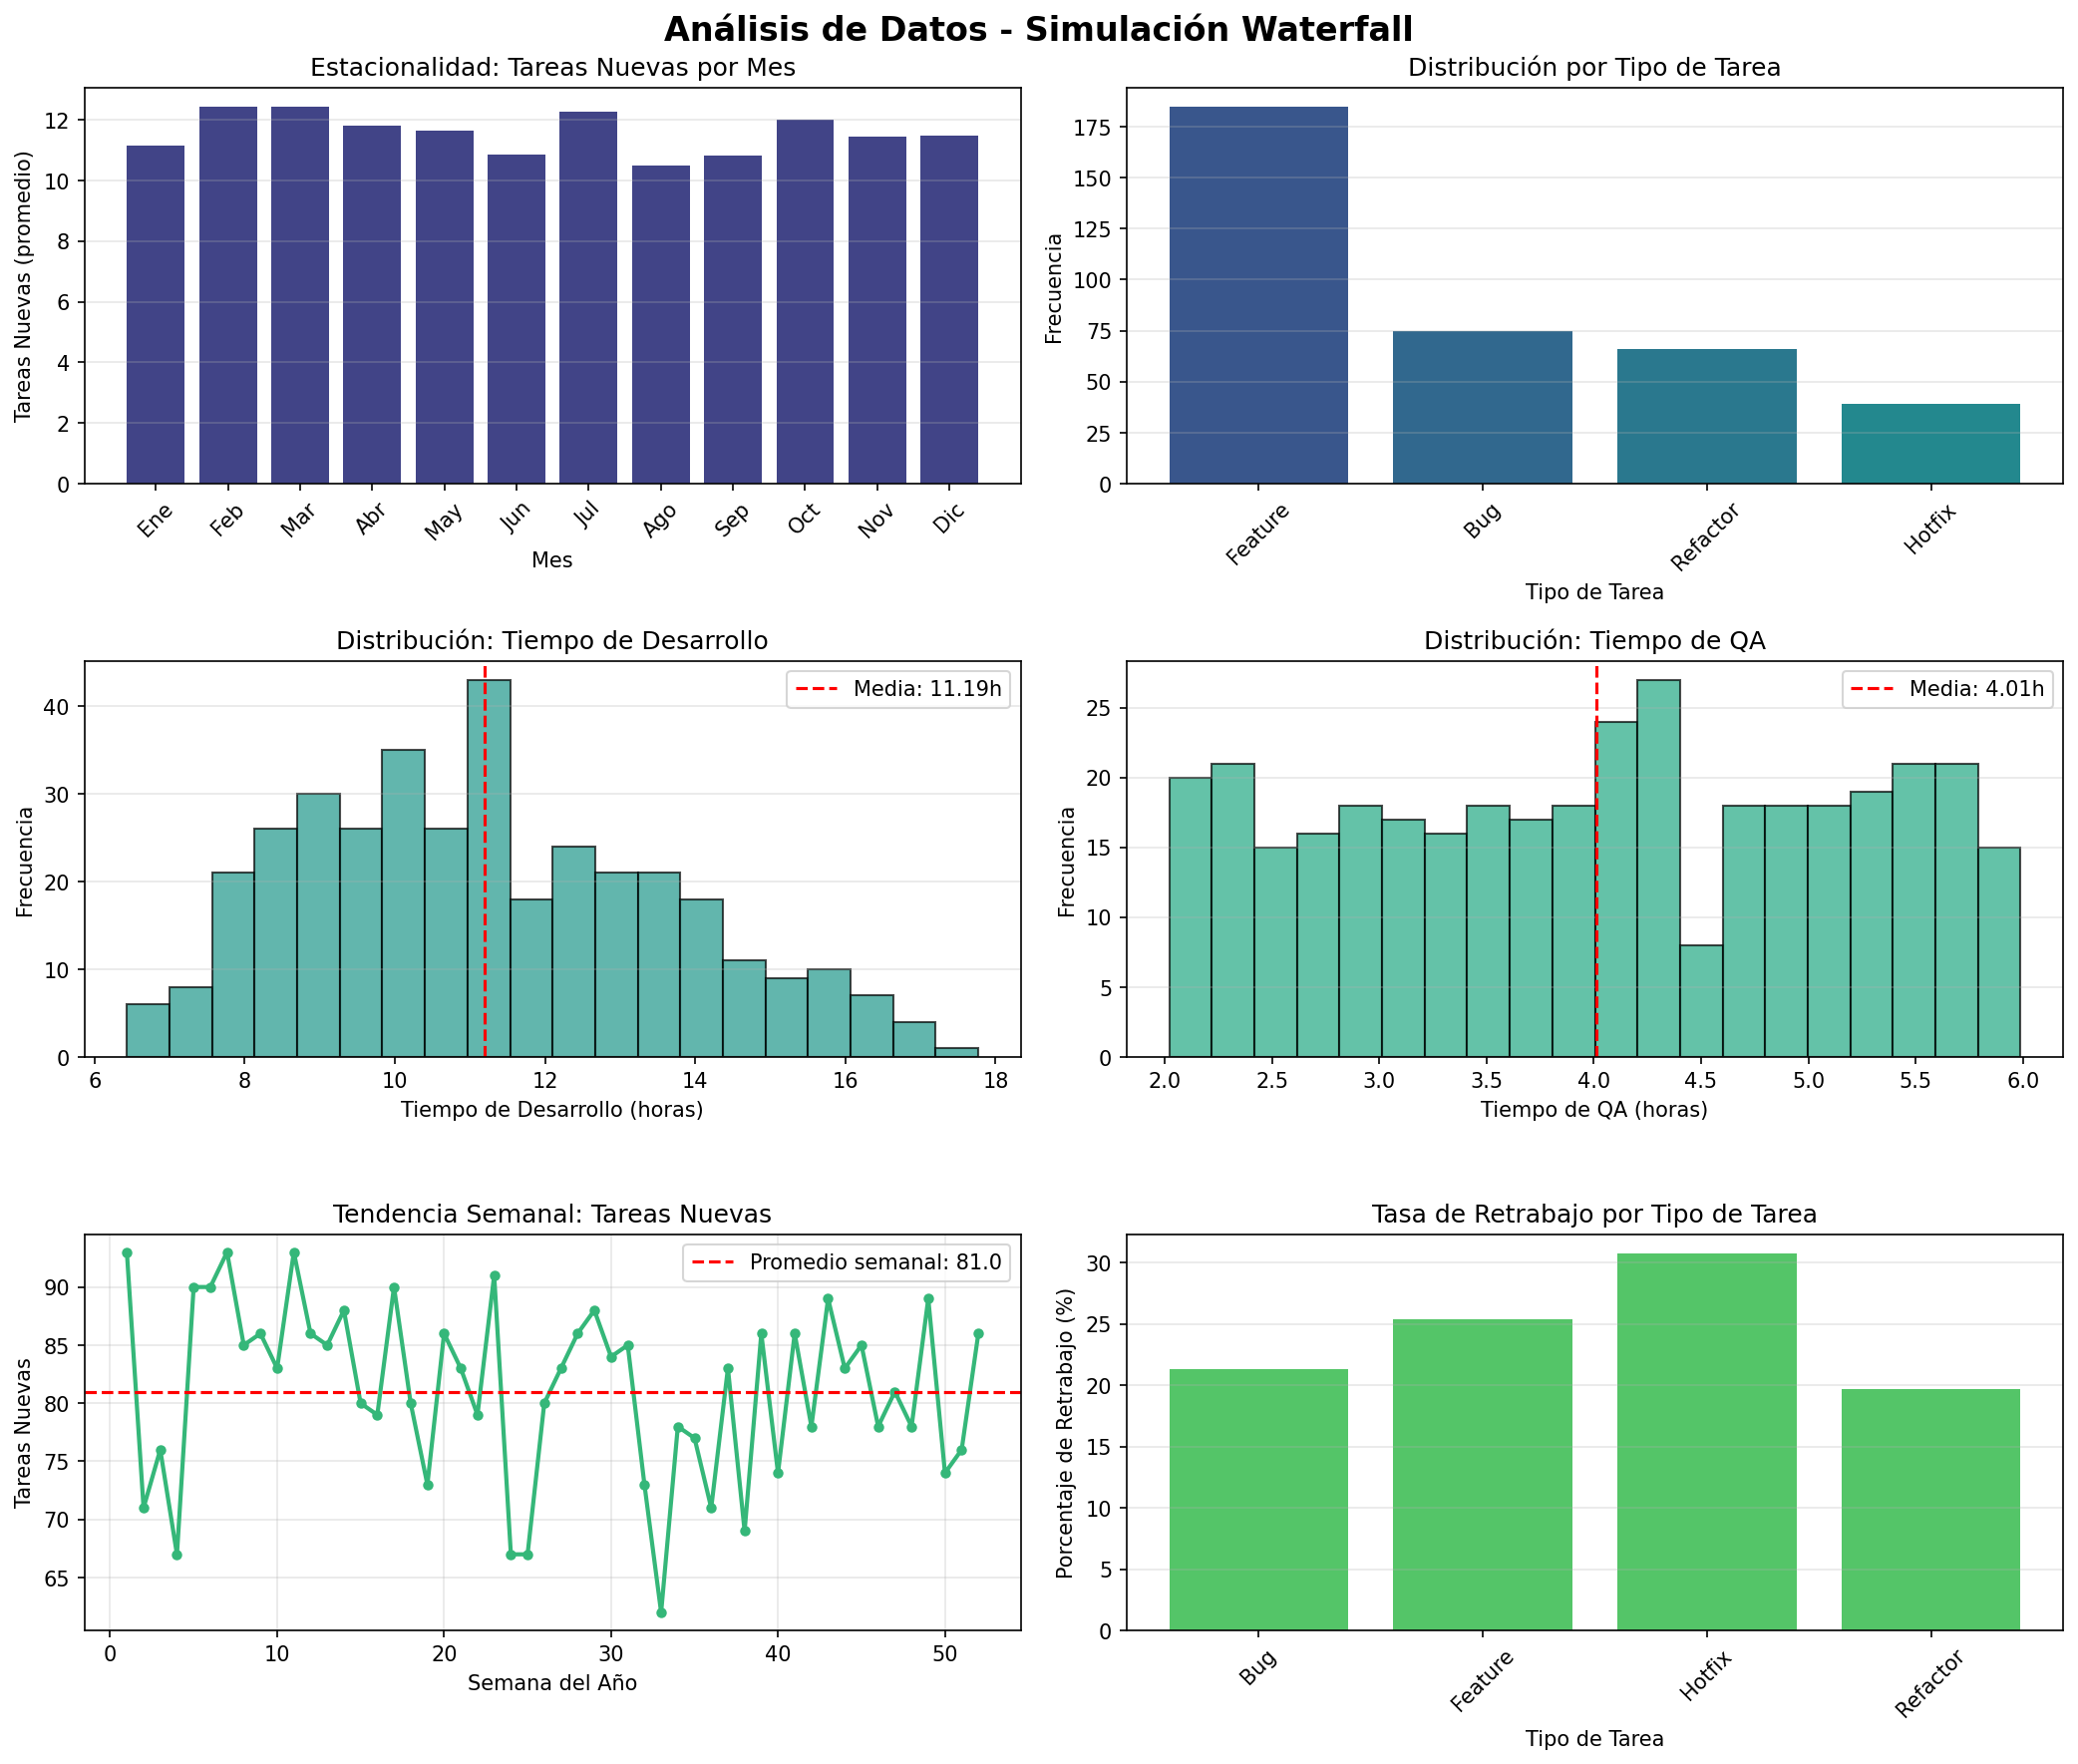
\includegraphics[width=\textwidth]{analisis_visualizacion.png}
  \caption{Análisis visual de patrones del proceso: estacionalidad mensual, distribución por tipo de tarea, histogramas de desarrollo y QA, tendencia semanal y retrabajo por tipo de tarea.}
  \label{fig:analisis-visual}
\end{figure}

La Figura~\ref{fig:distribuciones-ajustadas} muestra los histogramas con las curvas de densidad ajustadas para las cuatro variables continuas principales. El ajuste por el método de Kolmogorov--Smirnov determinó que la distribución Normal describe adecuadamente las llegadas ($D = 0{,}087$, $p > 0{,}05$) y el tiempo de QA ($D = 0{,}072$, $p > 0{,}05$), mientras que la Weibull fue la mejor opción para el tiempo de desarrollo ($k = 2{,}17$, $\lambda = 6{,}21$) y el tiempo de retrabajo ($k = 3{,}78$, $\lambda = 6{,}21$).

\begin{figure}[htbp]
  \centering
  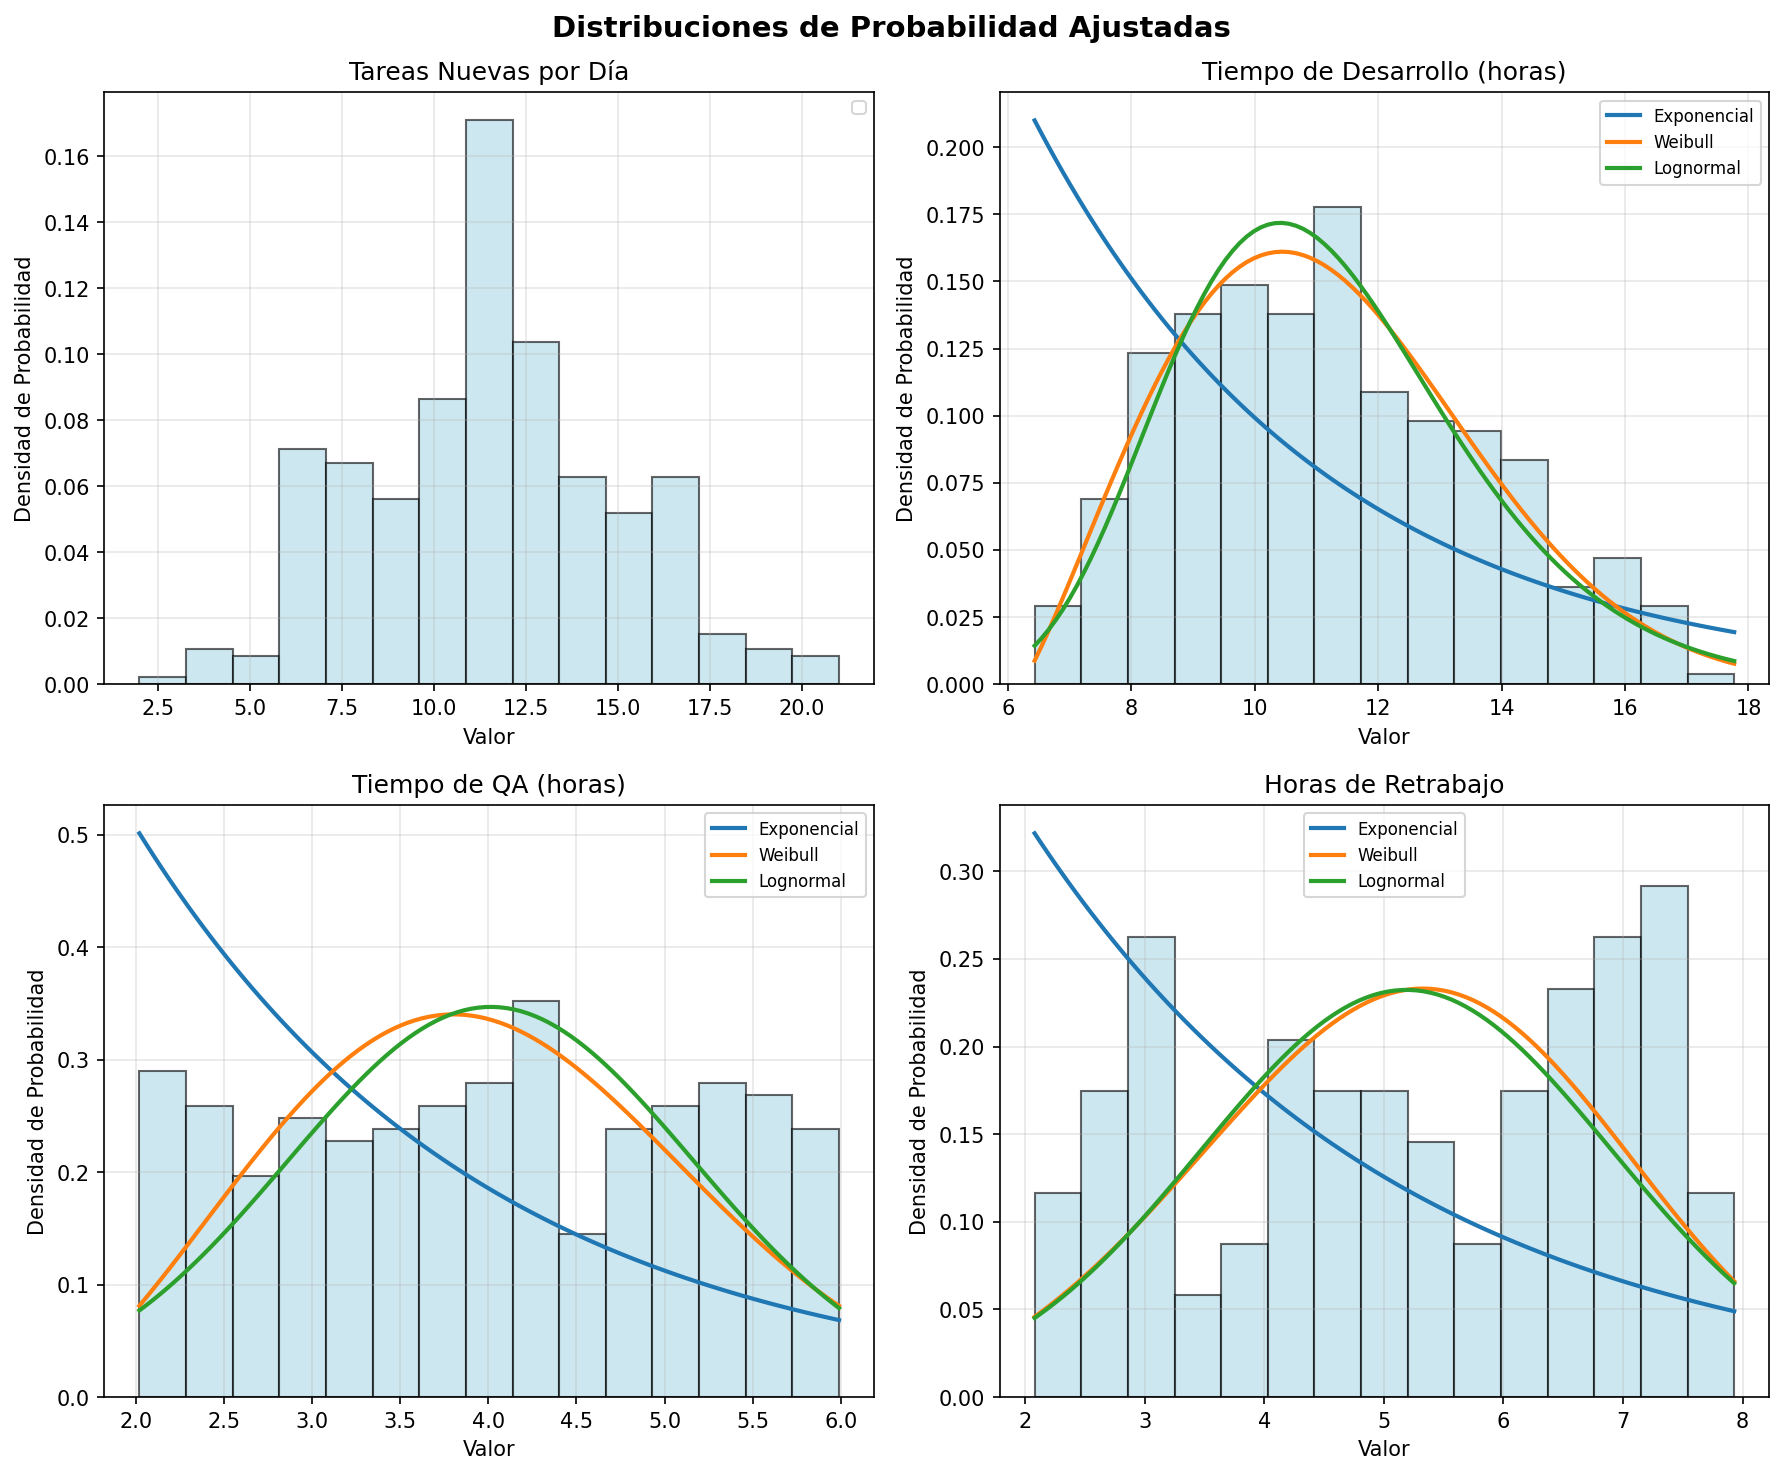
\includegraphics[width=\textwidth]{distribuciones_ajustadas.png}
  \caption{Histogramas con curvas de densidad ajustadas: llegadas diarias (Normal), tiempo de desarrollo (Weibull), tiempo de QA (Normal) y tiempo de retrabajo (Weibull).}
  \label{fig:distribuciones-ajustadas}
\end{figure}

Estos valores constituyen los parámetros de entrada del modelo de simulación descrito en la Sección~\ref{sec:metodologia}. La precisión del ajuste es fundamental para garantizar que el modelo FlexSim represente fielmente el comportamiento real del proceso y que los resultados de la simulación sean transferibles al contexto operativo original.

\end{document}
